\documentclass[aspectratio=169]{beamer}

% Language setup
\usepackage[magyar]{babel} % Babel for Hungarian
\usepackage[T1]{fontenc} % Output character encoding
\usepackage[utf8]{inputenc} % Input character encoding
\selectlanguage{magyar}

% Beamer styling setup
\usetheme{Boadilla}
\usecolortheme{default}
%\setbeamercolor{titlelike}{parent=structure,bg=gray!15}
\setbeamertemplate{navigation symbols}{}
\setbeamertemplate{caption}[numbered]
%

% Spacing setup
\setlength{\parindent}{0pt} % No paragraph indenting
\setlength{\parskip}{5pt} % Set spacing between paragraphs
\frenchspacing
\newcommand{\mkspace}{\vspace{19pt}}
\newcommand{\rmspace}{\vspace{-19pt}}
\newcommand{\emptyline}{\vspace{\baselineskip}}
%

% Dependency setup
\usepackage{tikz}
\usetikzlibrary{decorations.markings}
\usetikzlibrary{calc}
%

% Style setup
\usepackage{caption}
\captionsetup{format=plain, font=scriptsize, labelformat=empty}
%

% Notation setup
\usepackage{physics} % Braket notation

% Add qi.svg logo
\usepackage{svg}
\usepackage[absolute,overlay]{textpos}

% Newline in cell
\usepackage{makecell}

\author[Nemkin Viktória]{Nemkin Viktória}
\institute[]{
\begin{small}dr. Friedl Katalin\end{small}\\
\begin{footnotesize}Számítástudományi és Információelméleti Tanszék\end{footnotesize}
}
\title{Kvantumalgoritmusok bioinformatikai alkalmazása}
\subtitle{Protein folding \& Molecular docking}
\date{}

\begin{document}

\begin{frame}
\titlepage

\begin{textblock*}{150pt}(280pt,200pt) % {block width} (coords)
\includesvg[inkscape=overwrite,width=150pt]{./figures/qi.svg}
\end{textblock*}
\end{frame}

\begin{frame}
  \frametitle{Gráfbolyongások}
  
  \begin{itemize}
    \item Véletlen séta a gráf csúcsain (speciális Markov-lánc).
    \item Klasszikusan:
    \begin{itemize}
        \item Google kereső: PageRank
        \item Közelítő algoritmusok: SAT megoldó, részgráf keresése
    \end{itemize}
    \item Kvantumosan:
    \begin{itemize}
        \item Gyorsabb: $O(N^2) \rightarrow O(N)$ (elérés a szélére)
        \item Kvantum párhuzamosság
        \item Destruktív / konstruktív interferencia
        \item Korszerű, ma is aktívan kutatott, nem letisztult / kidolgozott
    \end{itemize}
  \end{itemize}
\end{frame}

\begin{frame}{Kvantumséták kutatása}
\begin{scriptsize}
Kvantum hardver: kevés qubit $\rightarrow$ Szimuláció klasszikus számítógépen
\begin{table}
\begin{tabular}{|l|l|l|l|l|l|l|l|l|l|}
  Package
& Frissítve
& Architektúra
& Gráfok
& \makecell[l]{Klasszikus\\szimuláció?}
& Kezdők számára?
\\ \hline

  \href{https://github.com/QWalk/mainline}{\color{blue}QWalk}
& 2018
& \makecell[l]{C++, optimalizációra\\kihegyezett}
& \makecell[l]{rács\\molekula-\\szerkezet}
& \makecell[c]{\texttimes}
& \makecell[l]{\texttimes: kvantum Monte\\Carlo elektronstruktúra\\számítások}
\\ \hline

  \href{https://github.com/Haixing-Hu/qwViz/}{\color{blue}QwViz}
& 2016
& C, szkript jellegű
& \makecell[l]{irányítatlan\\gráfok, mátrix\\kézzel megadva}
& \makecell[c]{\texttimes}
& \makecell[l]{\texttimes: C forráskód technikai}
\\ \hline

  \href{https://github.com/hiperwalk/hpwalk}{\color{blue}Hiperwalk}
& 2017\footnote{\scriptsize{}2021: Python 2 $\rightarrow$ 3 átállás}
& \makecell[l]{Python \& Neblina, szkript\\jellegű, nested if-ek}
& \makecell[l]{egyenes, kör\\rács, tórusz}
& \makecell[c]{\texttimes}
& \makecell[l]{\checkmark: saját bemeneti nyelv,\\de bővíteni nehéz}
\\ \hline

\href{https://github.com/iitis/QuantumWalk.jl}{\color{blue}QuantumWalk.jl}
& 2020
& \makecell[l]{Julia, szép architektúra\\de: Szegedy-féle sétára}
& \makecell[l]{irányított gráfok}
& \makecell[c]{\texttimes}
& \checkmark


\end{tabular}
\end{table}

Nem diszkrét séták:
\begin{itemize}
\item \href{https://github.com/josh146/pyctqw}{\color{blue}PyCTQW}: 2014, csak folytonos idejű szimuláció
\item \href{https://github.com/iitis/QSWalk.jl}{\color{blue}QSWalk.jl}: 2020, csak quantum stochastic walk szimuláció (generalizáció)
\end{itemize}

\end{scriptsize}
\end{frame}

\begin{frame}{Feladat}

\begin{columns}[t,onlytextwidth]
    \begin{column}{.5\textwidth}
      \begin{center}
        \textbf{Elméleti matematikai}
      \end{center}
      \begin{itemize}
          \item Markov-láncok, valószínűségszámítás
          \item Gráfelméleti algoritmusok: körlefedés, teljes párosítás
          \item Kvantuminformatika, komplex lineáris algebra
          \item Diszkrét idejű kvantumséták: position-coin notation, (arc notation, Szegedy-féle séta)
          \item Kvantummechanikából származtatva (Kempe): 1 dimenziós séta = részecske $\rightarrow$ hullámcsomag + spintől függő irány + detektálás valószínűsége
      \end{itemize}
    \end{column}
    \begin{column}{.5\textwidth}
      \begin{center}
         \textbf{Szoftvermérnöki}
      \end{center}
      \begin{itemize}
          \item Architekturális tervezés: Strategy minta
          \item Clean code elvek: Újrafelhasználhatóság, egységbe zárás, olvashatóság
          \item Futásidő és memóriahasználat optimalizálása: Szomszédossági orákulum
          \item Eszközök megválasztása:
          \begin{itemize}
            \item Nyelv: Python3
            \item Lineáris algebrai műveletek: Numpy
            \item Eredmények vizualizációja: Matplotlib
            \item Report fájl generálása: Latex
          \end{itemize}
      \end{itemize}
    \end{column}
  \end{columns}
\end{frame}

\begin{frame}
  \frametitle{1 dimenziós séta}
  \begin{figure}[H]
    \centering
    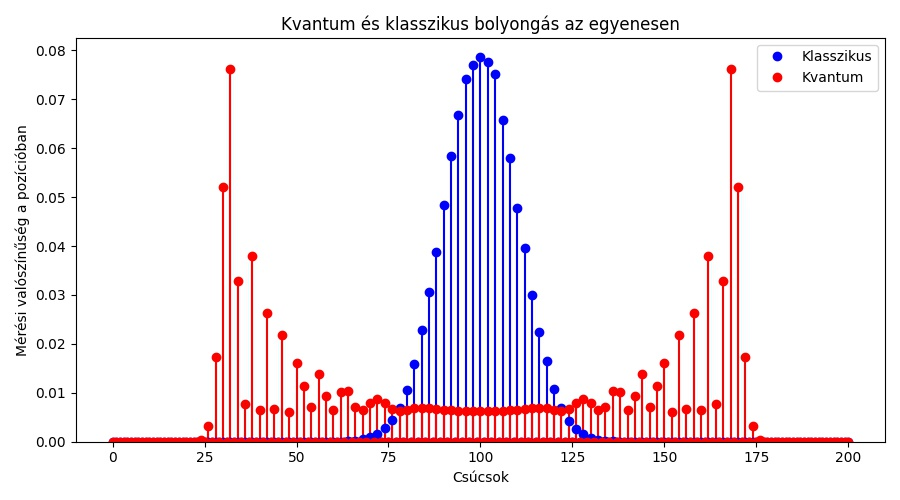
\includegraphics[width=0.9\linewidth]{./figures/teve.jpg}
  \end{figure}
\end{frame}

\begin{frame}
  \frametitle{Kvantumérme}
 
  \begin{columns}[t,onlytextwidth]
    \begin{column}{.5\textwidth}
     \begin{itemize}
    \item Kvantum regiszer: $\ket{c} \rightarrow$ \\ Érme aktuális állapota
    \item Evolúció operátor: $\ket{C} \rightarrow$
  \end{itemize}
      \begin{center}
    
    \textbf{Fourier} ($\omega = e^{\frac{2\pi{}i}{N}}$)

        \addvspace{10pt}

$\frac{1}{\sqrt{N}}
\begin{pmatrix}
  1 & 1 & 1 & \dots & 1 \\
  1 & \omega & \omega^2 & \dots & \omega^{N-1} \\
  1 & \omega^2 & \omega^4 & \dots & \omega^{2(N-1)} \\
  \vdots & \vdots & \vdots & \ddots & \vdots \\
  1 & \omega^{N-1} & \omega^{2(N-1)} & \dots & \omega^{(N-1)(N-1)}
\end{pmatrix}
$
    
    
    
      \end{center}

    \end{column}
    \begin{column}{.5\textwidth}
        \begin{center}
        
         \textbf{Hadamard}
        
        \addvspace{10pt}
        
$
   \mathbf{H} = \begin{pmatrix}
      \frac{1}{\sqrt{2}} & \frac{1}{\sqrt{2}}  \\
      \frac{1}{\sqrt{2}} & -\frac{1}{\sqrt{2}}
    \end{pmatrix}$

        \addvspace{10pt}
        
$\mathbf{H_n} = \mathbf{H}^{\otimes{}n}$


        \addvspace{10pt}
        
\textbf{Grover}
        
        \addvspace{10pt}
        
$
\begin{pmatrix}
      \frac{2}{N} - 1 & \frac{2}{N} & \dots  & \frac{2}{N} \\
      \frac{2}{N} & \frac{2}{N} - 1 & \dots  & \frac{2}{N} \\
      \vdots & \vdots & \ddots & \vdots \\
      \frac{2}{N} & \frac{2}{N} & \vdots & \frac{2}{N} - 1
    \end{pmatrix}
$


      \end{center}
    \end{column}
  \end{columns}
\end{frame}


\begin{frame}{Kvantum shift operátor: Saját munkám}
\begin{itemize}
    \item \textbf{Több egydimenziós érme + kvantum shift operátor $\rightarrow$ n dimenziós rács}
    \begin{itemize}
        \item Bizonyítottam, hogy a kvantum shift operátor felbomlik $n$ darab független $2$ dimenziós operátorra.
        \item Ezt felhasználva a memóriaigény lecsökkenthető:
        \begin{itemize}
            \item A $d$-től nem exponenciálisan, csak lineárisan függ.
            \item A futásidőt $d$-szeresére növelve a memóriaigény $d$-ben konstans.
        \end{itemize}
    \end{itemize}
    \item \textbf{Egy többdimenziós érme $\rightarrow$ d-reguláris gráf}
    \begin{itemize}
        \item Explicit unitér mátrixos felírás (függvények és implicit helyett).
        \item Bizonyítás: Shift operátor a gráf körlefedéséből (élszínosztályokból) kiindulva konstruálható
    \end{itemize}
\end{itemize}
\end{frame}

\begin{frame}
  \frametitle{1 dimenziós bolyongás}
  \begin{columns}[onlytextwidth]
    \begin{column}{.5\textwidth}
      \begin{figure}
        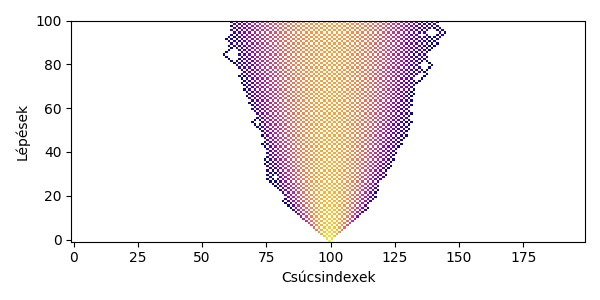
\includegraphics[width=\textwidth]{./figures/classical_simulation_short.jpg}
        \caption{\hspace{0.71cm}Klasszikus bolyongás}
      \end{figure}
    \end{column}
    \hfill
    \begin{column}{.5\textwidth}
      \begin{figure}
        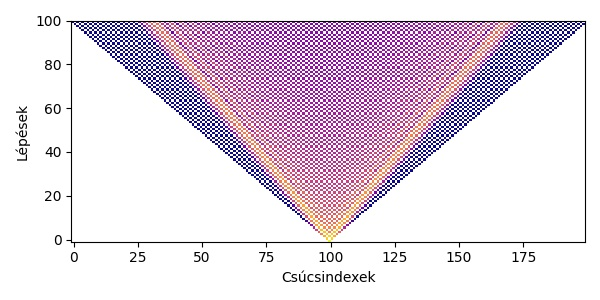
\includegraphics[width=\textwidth]{./figures/quantum_simulation_short.jpg}
        \caption{\hspace{0.73cm}Kvantum bolyongás}
      \end{figure}
    \end{column}
  \end{columns}
\end{frame}

\begin{frame}{1 dimenziós bolyongás körbeér}

  \begin{columns}[onlytextwidth]
    \begin{column}{.25\textwidth}
    \end{column}
    \begin{column}{.25\textwidth}
      \begin{figure}
        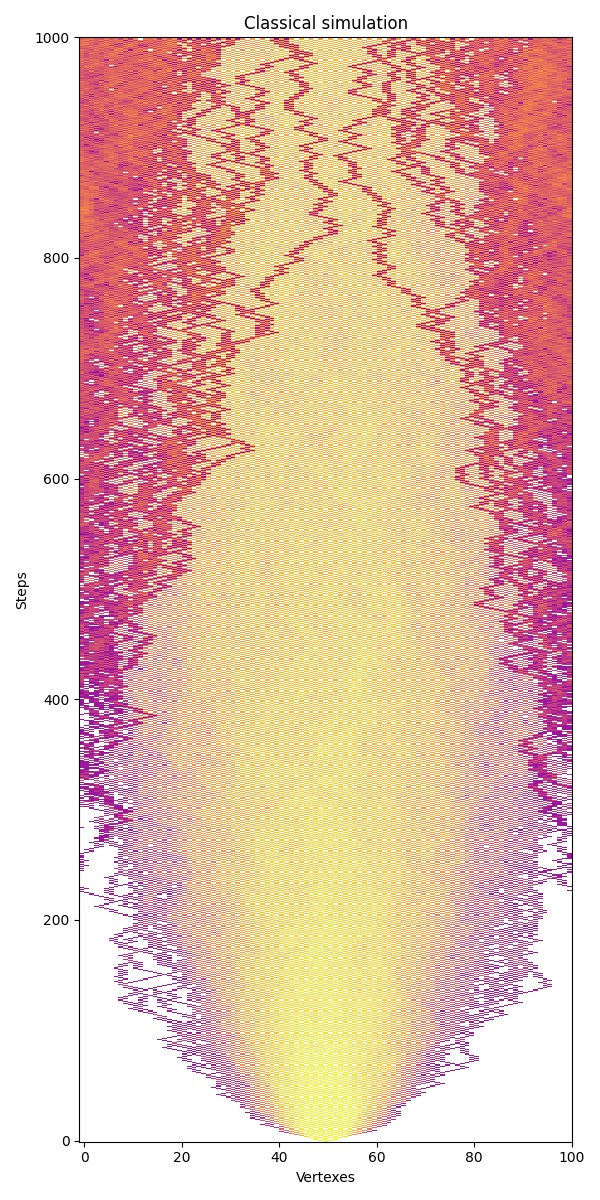
\includegraphics[width=0.9\textwidth]{./tdk_figures/results/path/classical.jpg}
      \end{figure}
    \end{column}
    \begin{column}{.25\textwidth}
      \begin{figure}
        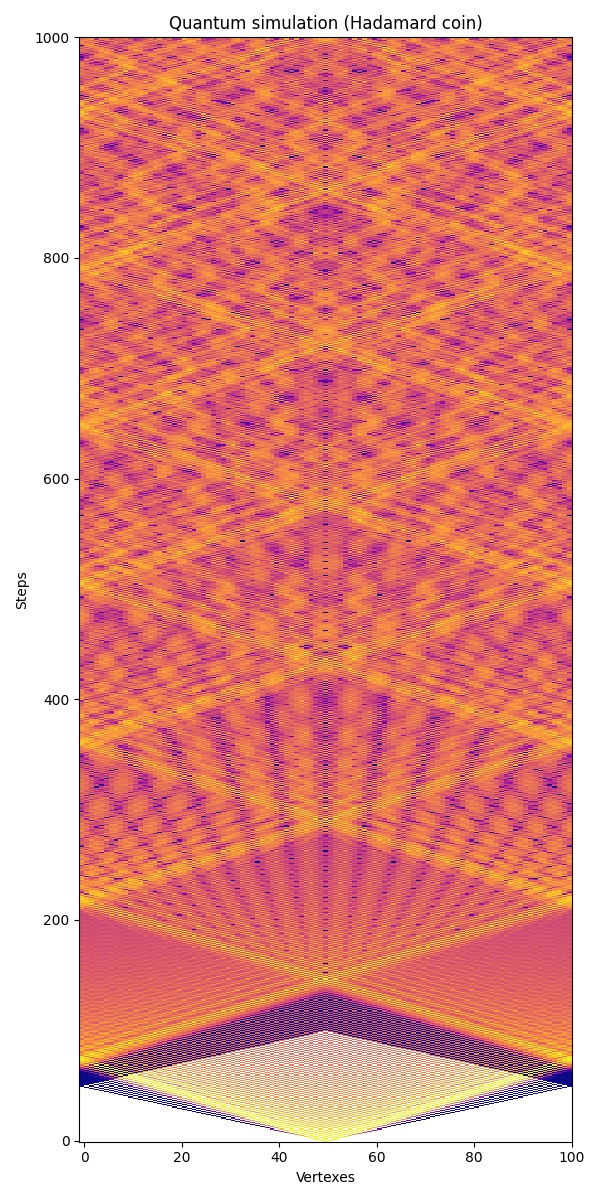
\includegraphics[width=0.9\textwidth]{./tdk_figures/results/path/hadamard.jpg}
      \end{figure}
    \end{column}
    \begin{column}{.25\textwidth}
    \end{column}
  \end{columns}
\end{frame}

\begin{frame}{Rácson bolyongás}

  \begin{columns}[onlytextwidth]
    \begin{column}{.23\textwidth}
      \begin{figure}
        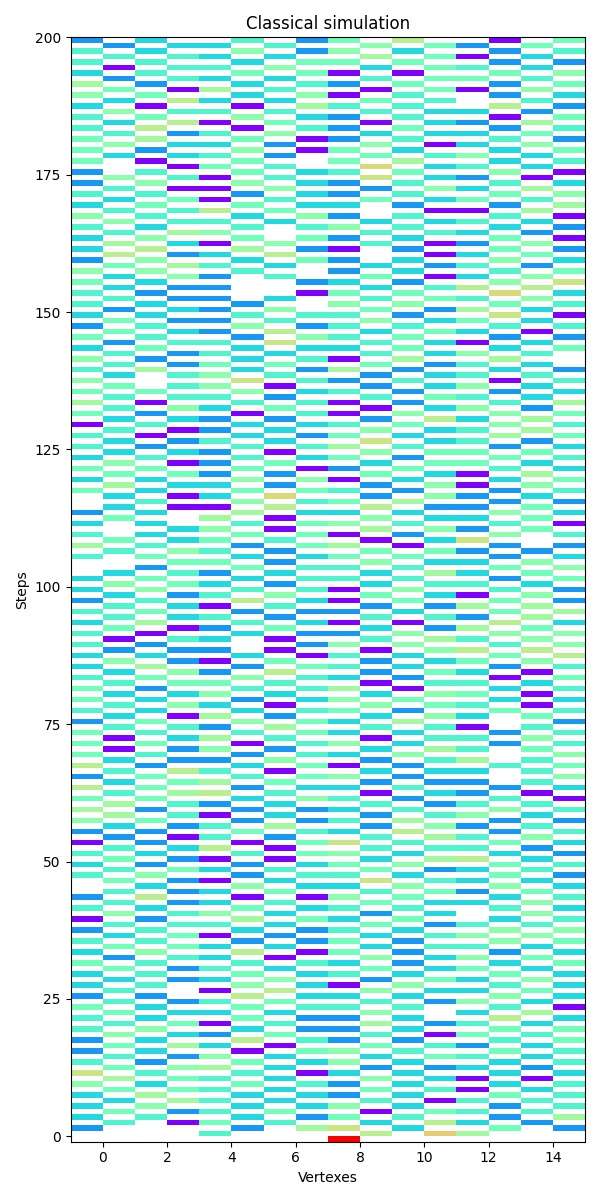
\includegraphics[width=0.9\textwidth]{./tdk_figures/results/grid/classical.jpg}
      \end{figure}
    \end{column}
    \begin{column}{.08\textwidth}
    \end{column}
    \begin{column}{.23\textwidth}
      \begin{figure}
        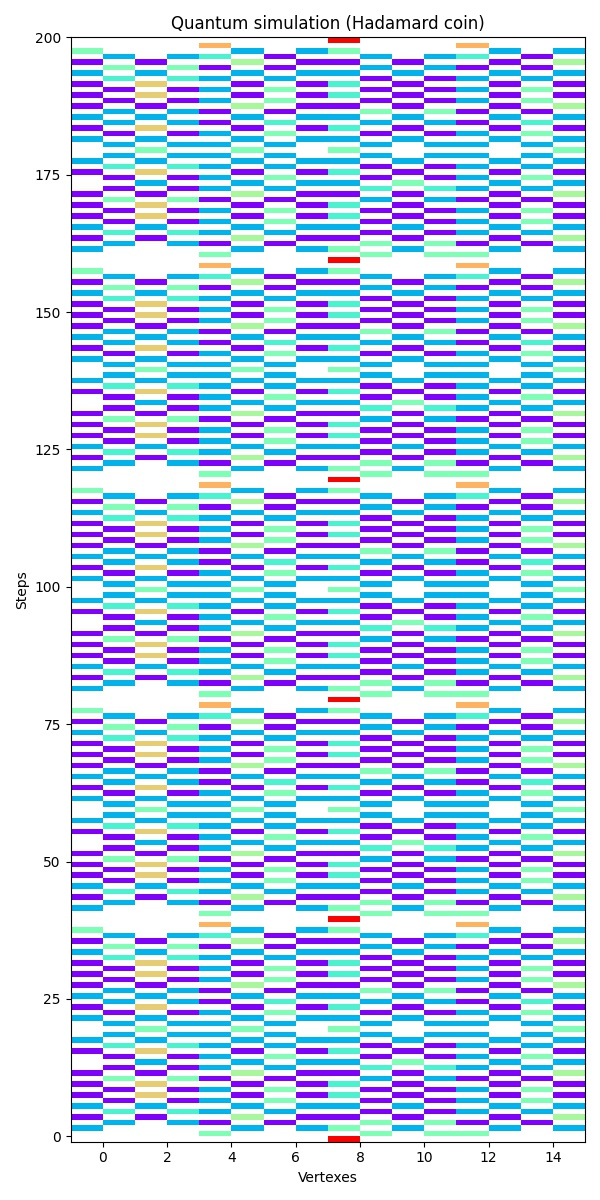
\includegraphics[width=0.9\textwidth]{./tdk_figures/results/grid/hadamard.jpg}
      \end{figure}
    \end{column}
     \begin{column}{.23\textwidth}
      \begin{figure}
        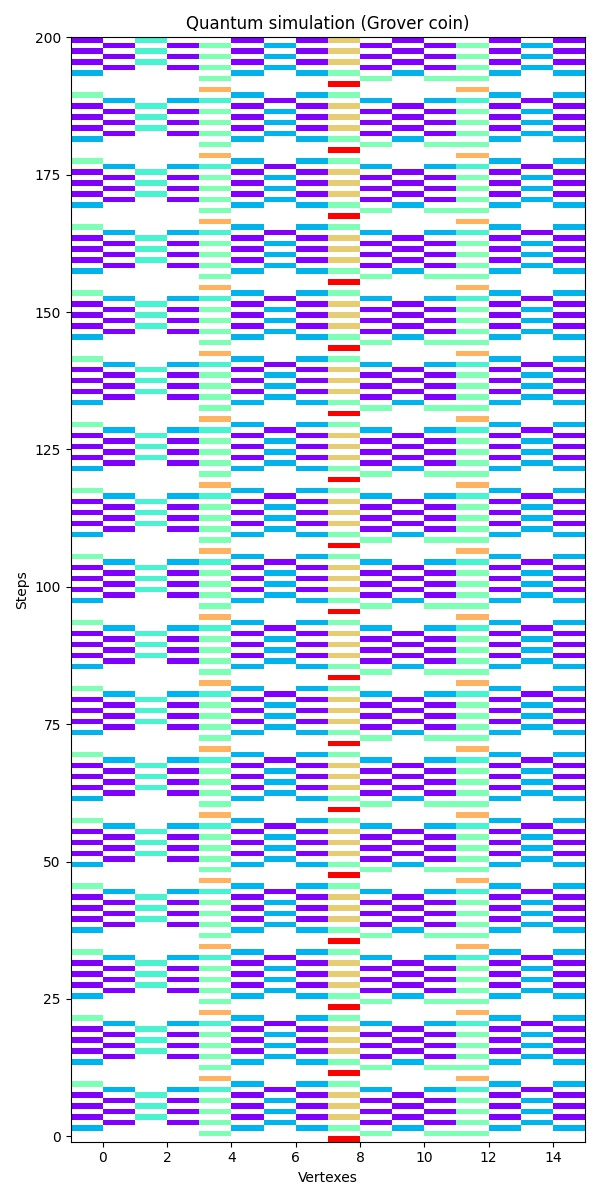
\includegraphics[width=0.9\textwidth]{./tdk_figures/results/grid/grover.jpg}
      \end{figure}
    \end{column}
    \begin{column}{.23\textwidth}
      \begin{figure}
        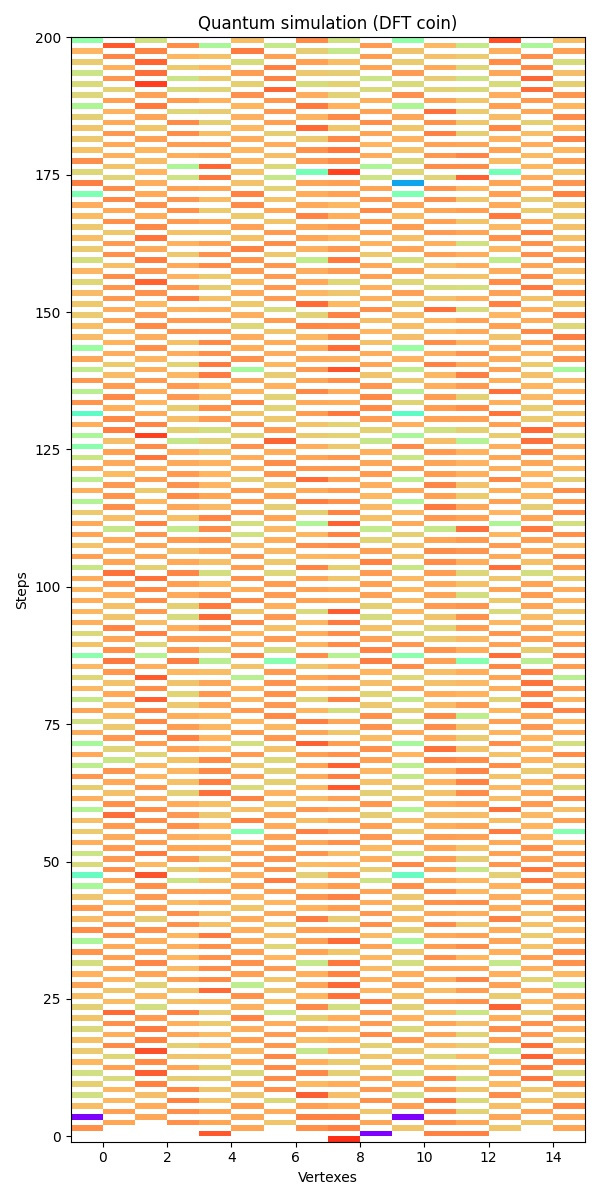
\includegraphics[width=0.9\textwidth]{./tdk_figures/results/grid/dft.jpg}
      \end{figure}
    \end{column}
  \end{columns}
\end{frame}

\begin{frame}{Hiperkockán bolyongás}

  \begin{columns}[onlytextwidth]
    \begin{column}{.23\textwidth}
      \begin{figure}
        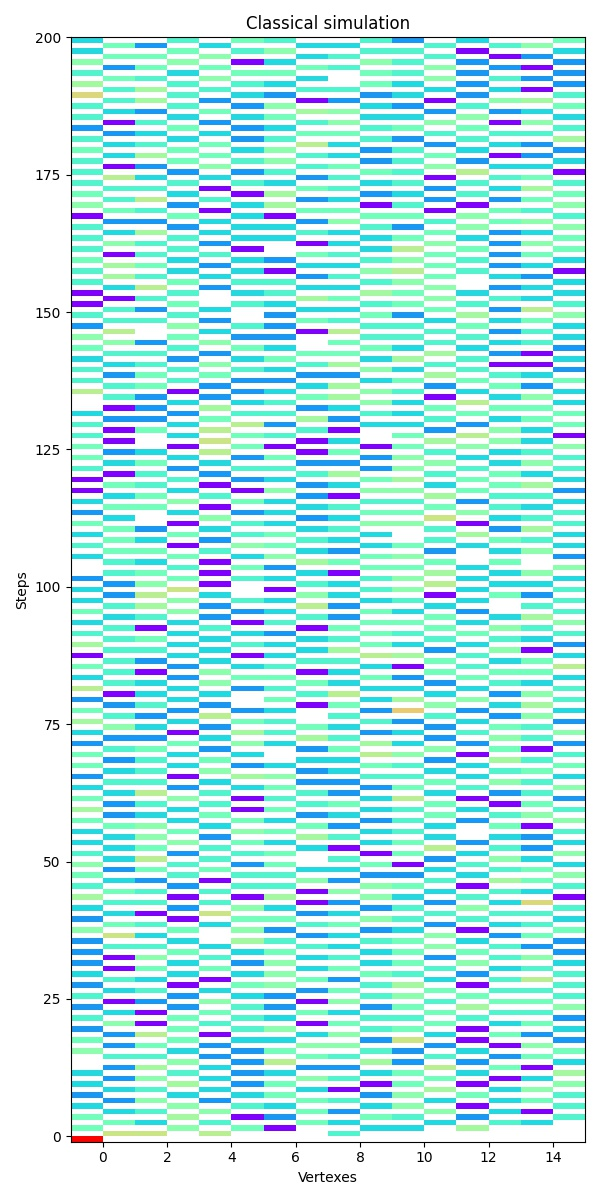
\includegraphics[width=0.9\textwidth]{./tdk_figures/results/hypercube/classical.jpg}
      \end{figure}
    \end{column}
    \begin{column}{.08\textwidth}
    \end{column}
    \begin{column}{.23\textwidth}
      \begin{figure}
        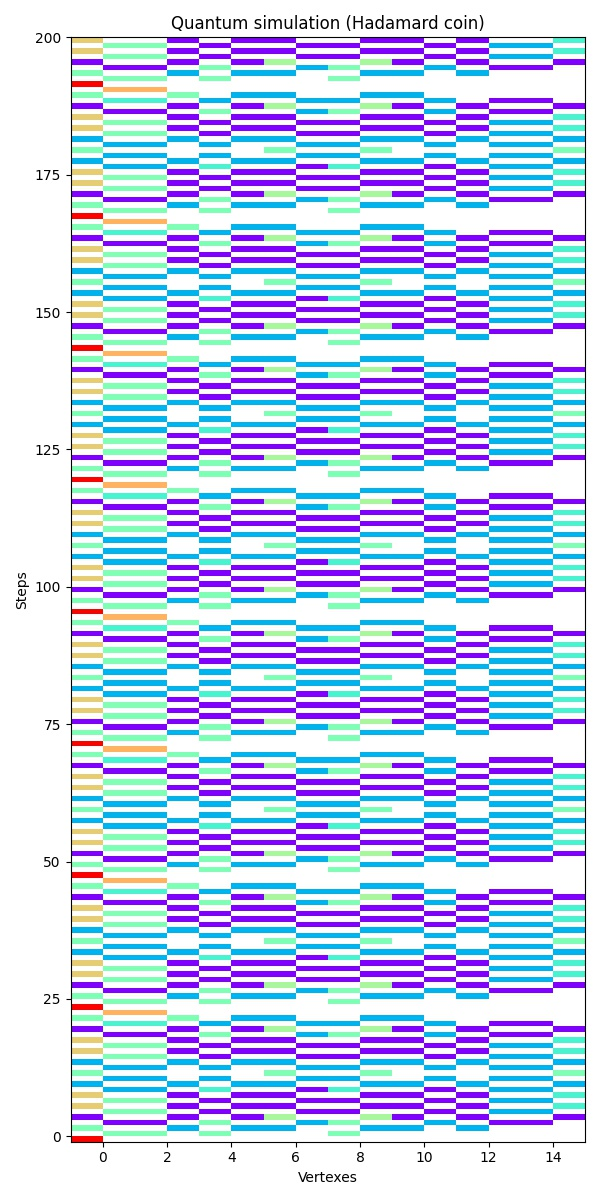
\includegraphics[width=0.9\textwidth]{./tdk_figures/results/hypercube/hadamard.jpg}
      \end{figure}
    \end{column}
    \begin{column}{.23\textwidth}
      \begin{figure}
        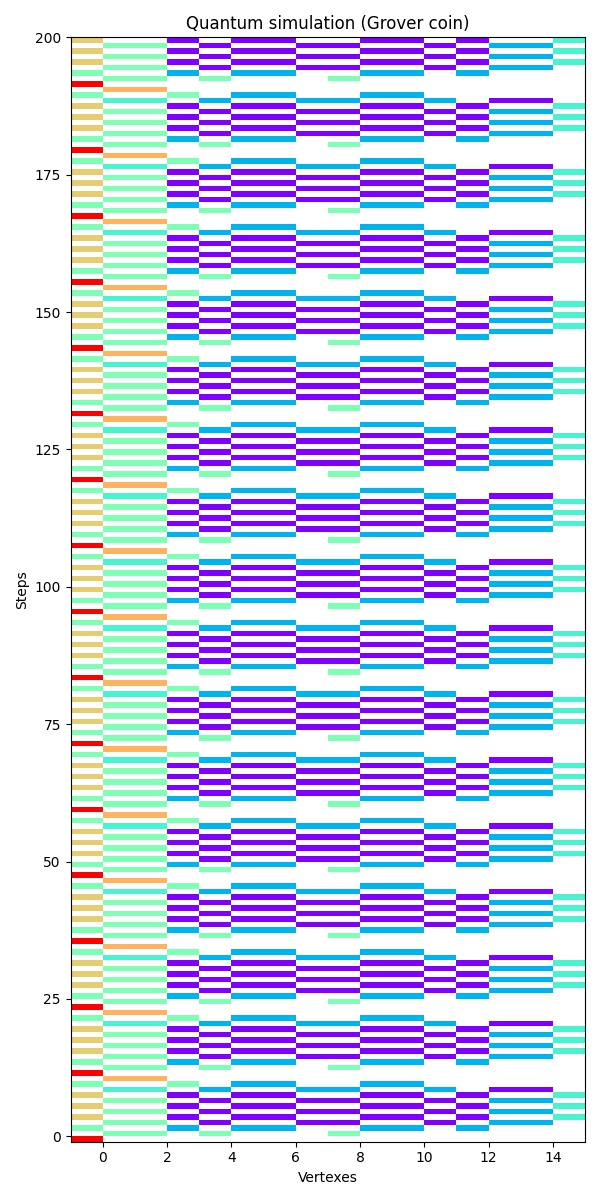
\includegraphics[width=0.9\textwidth]{./tdk_figures/results/hypercube/grover.jpg}
      \end{figure}
    \end{column}
    \begin{column}{.23\textwidth}
      \begin{figure}
        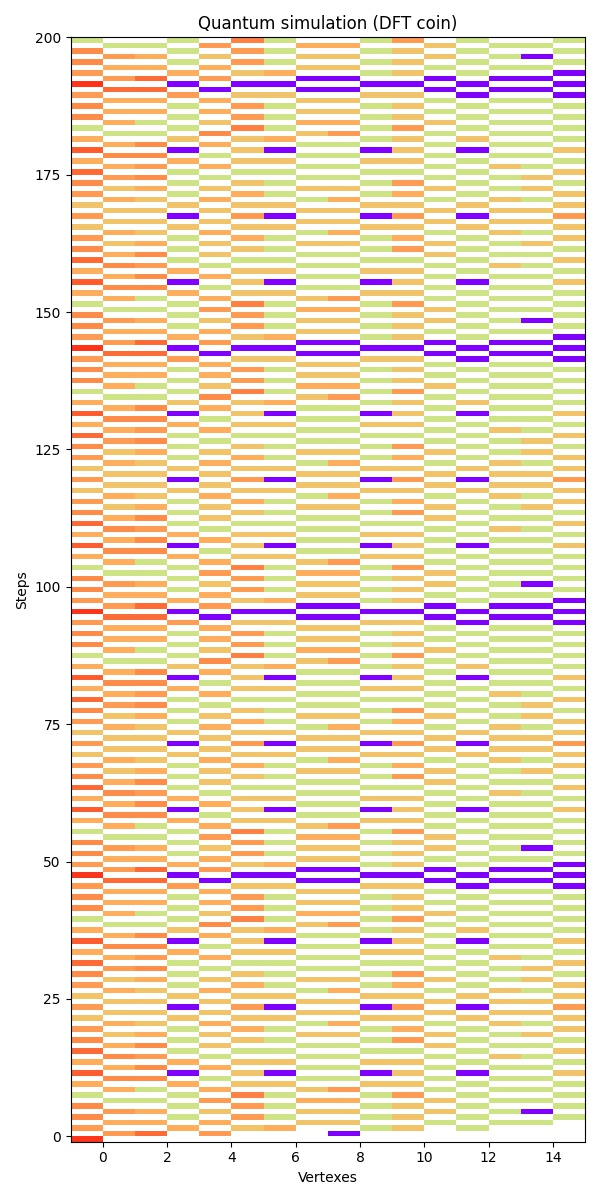
\includegraphics[width=0.9\textwidth]{./tdk_figures/results/hypercube/dft.jpg}
      \end{figure}
    \end{column}
  \end{columns}
\end{frame}

\begin{frame}{Kitekintés}
\begin{itemize}
    \item Szimulátor szoftver: \url{github.com/nemkin/quantum} (open source, MIT licensz)
    \item Kutatási irány:
    \begin{itemize}
        \item kvantumséta alapú keresési algoritmus
        \item klasszikusan NP-teljes problémák (protein folding) megoldására
    \end{itemize}
\end{itemize}
\end{frame}

\begin{frame}{Bíráló kérdései}

\begin{itemize}
    \item Miként értelmezhető a hitting time ábrákon a görbék folytonossága a vízszintes tengely mentén?
    \begin{itemize}
        \item Nem a megfelelő grafikontípust választottam a diszkrét jellegű adatok szemléltetésére.
    \end{itemize}
     \begin{figure}[H]
        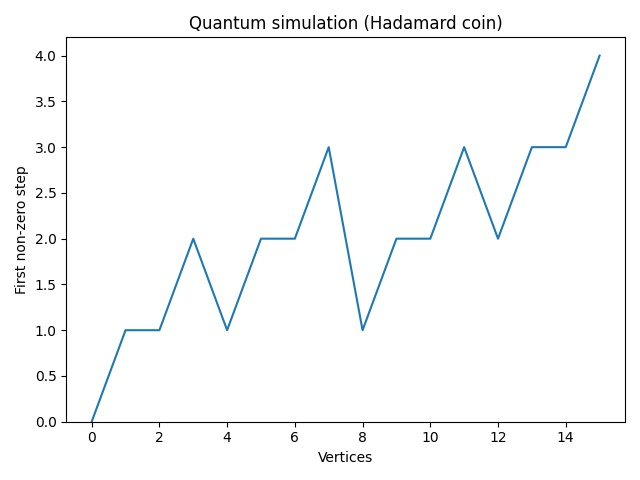
\includegraphics[width=0.5\linewidth]{./tdk_figures/results/hypercube/hadamard_hitting_time.jpg}
      \end{figure}
\end{itemize}

\end{frame}


\begin{frame}{Bíráló kérdései}

\begin{itemize}
    \item Mi a TDK dolgozat elsődleges célja? A kvantumséta kutatása, vagy egy szimulátor írása, amely alkalmas a kvantumsétákkal kapcsolatos kutatások támogatására?
    \begin{itemize}
        \item A TDK dolgozatom célja a kvantum shift operátorral kapcsolatos 2 elméleti eredmény bemutatása, továbbá 
        ezekre építve a szimulátor szoftver implementálása volt. Hosszú távon ezt a szoftvert felhasználva szeretnék kvantumsétákra alapuló kvantumos keresőalgoritmusok kutatásával foglalkozni.
    \end{itemize}
    \item "Mátrix elemzés" a szerző által ismert szimulátorokról a dolgozatban javasolt 5 értékelési szempont alapján.
    \begin{itemize}
        \item A 3. dián látható a dolgozatból hiányzó mátrix elemzés.
    \end{itemize}
\end{itemize}

\end{frame}

\end{document}